\section{Model predictions errors for provinces in Vietnam}

Finally, we evaluated the performance of the different versions of the model when applied to data for different provinces in Vietnam.
Comparable to the previous results obtained when experimenting with country-level data and \gls{US} counties data, all versions were capable of predicting future cases for all compartments with relatively high accuracy at most locations except for Ho Chi Minh city.
With Vietnam provinces data, it was found that all the versions performed best for up to 14 days before the accuracy started to fall off.
Moreover, the results also suggested that the covariates that we had chosen did not have a positive effect on the long-term forecasting ability of the model.

Regarding predictions errors for the number of deaths in \autoref{tab:errors-vn-provinces-deaths}, across all metrics for the 7-day forecast horizon, the baseline model achieved the lowest predictions errors for three provinces Binh Duong, Dong Nai, and Ho Chi Minh city while the second version performed best on data for Long An.
On all the considered error metrics, for the 14-day, 21-day, and 28-day forecast horizons, the baseline model performed best on data for Dong Nai and Ho Chi Minh city whereas the second version made the best predictions for Binh Duong and Long An.
When predicting the number of deaths for Ho Chi Minh city, all three versions did not make good predictions where the \gls{MAPE} value was lowest at $35$\% for the 7-day forecast and highest at $46$\% for the 28-day forecast.
Furthermore, the baseline model and the third version also made bad predictions for the number of deaths for Long An where the lowest \gls{MAPE} was $21$\% for the 7-day forecast and the highest \gls{MAPE} was $45$\% for the 28-day forecast.

Looking at \autoref{tab:errors-vn-provinces-new-cases}, it can be seen that across all metrics for the 7-day forecast horizon, the baseline model had the lowest predictions errors for Ho Chi Minh city, the second version had the lowest predictions errors for Binh Duong, and the third version performed best for Dong Nai and Long An.
Moving on to the 14-day forecast horizon, across all metrics, the baseline model now achieved the lowest predictions errors for Dong Nai and Ho Chi Minh city, the second version had the best performance for Binh Duong, and the third version had the best performance for Long An.
Next with the 21-day forecast horizon, the baseline model continued to have the best performance across all metrics for Dong Nai and Ho Chi Minh city.
While the second version had the lowest \gls{MAE} for Binh Duong city, the predictions with the lowest \gls{MAPE} and lowest \gls{RMSE} were made by the third version.
In addition, the third version also had the lowest predictions errors for Long An across all metrics.
With the 28-day forecast horizon, the baseline model had the lowest predictions errors for Dong Nai across all metrics, however, for Ho Chi Minh city, the model only achieved the lowest \gls{MAE} and \gls{MAPE} while the second version had the lowest \gls{RMSE}.
Finally, the third version performed best for Binh Duong and Long An across all metrics.
Except for the baseline model's predictions for Dong Nai, all other predictions for the number of new cases for provinces in Vietnam had relatively high errors, especially with larger forecast horizons.
Here predictions' accuracy deteriorated when predicting with a horizon larger than 14 days where the \gls{MAPE} value was higher than $20$\% across all locations.

On the predictions for the number of cumulative cases, \autoref{tab:errors-vn-provinces-total-cases} shows that for Binh Duong, the baseline model had the lowest predictions errors across all metrics for the 7-day horizon, the second version had the lowest predictions errors across all metrics for the 14-day and 21-day horizon, and the third version had the lowest predictions errors across all metrics for the 28-day horizon.
For Dong Nai, the third version performed best across all metrics for the 7-day and 14-day horizon, however, with the 21-day horizon, the third version only had the lowest \gls{MAPE} while the lowest \gls{MAE} and lowest \gls{RMSE} were held by the baseline model.
In addition, the baseline model also had the best performance across all metrics for Dong Nai with the 28-day horizon.
For Ho Chi Minh city, the third version made the best predictions across all metrics for the 7-day horizon, while the baseline model was best across all metrics for the 14-day, 21-day, and 28-day horizons.
Lastly, for Long An, the third version had the best performance across all metrics and horizons.

Overall, all three versions had a good out-of-sample performance for the number of deaths and the number of cumulative when extrapolated from the training period.
Nonetheless, the model predictions errors for the number of new cases were still high, and in the case of Ho Chi Minh city, as shown in \autoref{fig:pred-vn-provinces}, all versions completely failed to capture the trend of the new cases.
Similar to the experiments with \gls{US} counties, it was likely that the model's performance was dependent on the characteristics of the locations that were modeled, and the encoded covariates provided little to no help in improving the model out-of-sample performance.

% ERRORS

\begin{landscape}
\begin{table}[!htb]
    \centering
    \begin{tabular}{| c | c | c | c | c | c | c | c | c | c | c |}
        \multirow{2}{*}{Days}
            & \multirow{2}{*}{Loc.}
            & \multicolumn{3}{c |}{Baseline}
            & \multicolumn{3}{c |}{2nd. Version}
            & \multicolumn{3}{c |}{3rd. Version} \\ \cline{3-11}
            & & MAE & MAPE & RMSE & MAE & MAPE & RMSE & MAE & MAPE & RMSE \\ \hline\hline

        \multirow{4}{*}{7}
            & Binh Duong & \textbf{95.426} & \textbf{5.812} & \textbf{98.695} & 100.100 & 6.106 & 102.736 & 121.271 & 7.385 & 125.535 \\
            & Dong Nai & \textbf{70.096} & \textbf{16.939} & \textbf{70.288} & 94.131 & 22.727 & 94.283 & 77.339 & 18.677 & 77.493 \\
            & Ho Chi Minh city & \textbf{969.400} & \textbf{35.439} & \textbf{991.778} & 976.721 & 35.690 & 999.832 & 1015.894 & 37.060 & 1042.086 \\
            & Long An & 94.571 & 33.788 & 95.339 & \textbf{8.248} & \textbf{2.931} & \textbf{8.550} & 61.189 & 21.732 & 63.484 \\ \hline

        \multirow{4}{*}{14}
            & Binh Duong & 139.067 & 7.795 & 147.809 & \textbf{138.019} & \textbf{7.764} & \textbf{144.724} & 176.025 & 9.869 & 186.921 \\
            & Dong Nai & \textbf{59.087} & \textbf{13.976} & \textbf{60.270} & 87.745 & 20.673 & 88.071 & 70.580 & 16.639 & 71.003 \\
            & Ho Chi Minh city & \textbf{1403.959} & \textbf{38.084} & \textbf{1489.430} & 1423.473 & 38.555 & 1512.527 & 1515.313 & 40.813 & 1619.890 \\
            & Long An & 115.136 & 38.395 & 117.520 & \textbf{11.775} & \textbf{3.890} & \textbf{12.432} & 92.512 & 30.445 & 99.238 \\ \hline

        \multirow{4}{*}{21}
            & Binh Duong & 177.847 & 9.335 & 190.719 & \textbf{168.792} & \textbf{8.910} & \textbf{177.966} & 223.925 & 11.759 & 239.736 \\
            & Dong Nai & \textbf{55.633} & \textbf{12.716} & \textbf{56.685} & 87.775 & 19.906 & 87.995 & 72.183 & 16.345 & 72.517 \\
            & Ho Chi Minh city & \textbf{1891.890} & \textbf{40.052} & \textbf{2062.596} & 1926.393 & 40.695 & 2104.055 & 2095.582 & 43.845 & 2309.499 \\
            & Long An & 134.235 & 42.112 & 138.380 & \textbf{14.507} & \textbf{4.507} & \textbf{15.372} & 124.800 & 38.414 & 136.510 \\ \hline

        \multirow{4}{*}{28}
            & Binh Duong & 203.904 & 10.232 & 217.207 & \textbf{185.288} & \textbf{9.373} & \textbf{193.737} & 257.546 & 12.925 & 274.293 \\
            & Dong Nai & \textbf{52.644} & \textbf{11.686} & \textbf{53.744} & 87.106 & 19.115 & 87.288 & 74.530 & 16.270 & 74.884 \\
            & Ho Chi Minh city & \textbf{2387.155} & \textbf{41.454} & \textbf{2637.652} & 2434.133 & 42.186 & 2693.007 & 2701.371 & 46.196 & 3022.084 \\
            & Long An & 151.608 & 45.047 & 157.341 & \textbf{16.404} & \textbf{4.841} & \textbf{17.303} & 157.136 & 45.593 & 173.810 \\ \hline
    \end{tabular}
    \caption{Out-of-sample errors of the model's predictions on the number of deaths for the provinces in Vietnam. The lowest errors for each evaluation metrics at each location are highlighted.}
    \label{tab:errors-vn-provinces-deaths}
\end{table}
\end{landscape}

\begin{landscape}
\begin{table}[!htb]
    \centering
    \begin{tabular}{| c | c | c | c | c | c | c | c | c | c | c |}
        \multirow{2}{*}{Days}
            & \multirow{2}{*}{Loc.}
            & \multicolumn{3}{c |}{Baseline}
            & \multicolumn{3}{c |}{2nd. Version}
            & \multicolumn{3}{c |}{3rd. Version} \\ \cline{3-11}
            & & MAE & MAPE & RMSE & MAE & MAPE & RMSE & MAE & MAPE & RMSE \\
        \hline\hline

        \multirow{4}{*}{7}
            & Binh Duong & 258.212 & 8.744 & 299.194 & \textbf{116.056} & \textbf{4.086} & \textbf{164.898} & 296.040 & 9.960 & 330.132 \\
            & Dong Nai & 130.533 & 17.341 & 135.187 & 209.730 & 27.792 & 214.491 & \textbf{39.442} & \textbf{5.266} & \textbf{49.236} \\
            & Ho Chi Minh city & \textbf{139.151} & \textbf{3.560} & \textbf{163.295} & 376.279 & 9.647 & 394.165 & 705.167 & 18.114 & 723.858 \\
            & Long An & 189.861 & 33.532 & 200.279 & 188.479 & 33.290 & 198.773 & \textbf{157.530} & \textbf{27.707} & \textbf{168.869} \\ \hline

        \multirow{4}{*}{14}
            & Binh Duong & 508.485 & 16.627 & 597.647 & \textbf{205.217} & \textbf{6.720} & \textbf{267.533} & 545.052 & 17.835 & 626.841 \\
            & Dong Nai & \textbf{84.028} & \textbf{11.122} & \textbf{103.395} & 179.143 & 23.323 & 186.383 & 133.415 & 16.778 & 169.034 \\
            & Ho Chi Minh city & \textbf{379.416} & \textbf{9.804} & \textbf{466.377} & 600.225 & 15.498 & 651.818 & 989.250 & 25.554 & 1040.354 \\
            & Long An & 199.785 & 36.232 & 211.350 & 197.566 & 35.802 & 209.171 & \textbf{163.229} & \textbf{29.231} & \textbf{176.954} \\ \hline

        \multirow{4}{*}{21}
            & Binh Duong & 514.164 & 25.439 & 596.107 & \textbf{500.765} & 32.829 & 695.279 & 518.767 & \textbf{24.589} & \textbf{594.628} \\
            & Dong Nai & \textbf{63.199} & \textbf{8.373} & \textbf{85.472} & 173.204 & 22.846 & 178.936 & 174.459 & 22.671 & 202.875 \\
            & Ho Chi Minh city & \textbf{742.775} & \textbf{17.905} & \textbf{960.595} & 902.403 & 22.027 & 1040.717 & 1338.583 & 32.902 & 1468.122 \\
            & Long An & 153.175 & 30.224 & 176.074 & 150.502 & 29.573 & 173.932 & \textbf{112.808} & \textbf{20.656} & \textbf{144.752} \\ \hline

        \multirow{4}{*}{28}
            & Binh Duong & 650.869 & 59.526 & 741.151 & 787.829 & 87.134 & 1021.467 & \textbf{623.044} & \textbf{54.074} & \textbf{696.459} \\
            & Dong Nai & \textbf{51.988} & \textbf{7.033} & \textbf{74.758} & 177.252 & 24.773 & 181.688 & 179.379 & 24.798 & 200.903 \\
            & Ho Chi Minh city & \textbf{1297.598} & \textbf{27.166} & 1713.583 & 1388.426 & 29.725 & \textbf{1697.844} & 1863.602 & 40.654 & 2149.100 \\
            & Long An & 118.454 & 24.197 & 152.753 & 116.804 & 23.893 & 150.918 & \textbf{98.185} & \textbf{21.637} & \textbf{128.612} \\ \hline
    \end{tabular}
    \caption{Out-of-sample errors of the model's predictions on the number of new cases for the provinces in Vietnam. The lowest errors for each evaluation metrics at each location are highlighted.}
    \label{tab:errors-vn-provinces-new-cases}
\end{table}
\end{landscape}

\begin{landscape}
\begin{table}[!htb]
    \centering
    \begin{tabular}{| c | c | c | c | c | c | c | c | c | c | c |}
        \multirow{2}{*}{Days}
            & \multirow{2}{*}{Loc.}
            & \multicolumn{3}{c |}{Baseline}
            & \multicolumn{3}{c |}{2nd. Version}
            & \multicolumn{3}{c |}{3rd. Version} \\ \cline{3-11}
            & & MAE & MAPE & RMSE & MAE & MAPE & RMSE & MAE & MAPE & RMSE \\ \hline\hline

        \multirow{4}{*}{7}
            & Binh Duong & \textbf{543.123} & \textbf{0.300} & \textbf{669.448} & 1080.846 & 0.605 & 1092.888 & 2716.160 & 1.539 & 2807.759 \\
            & Dong Nai & 925.781 & 2.478 & 968.738 & 1151.564 & 3.071 & 1239.187 & \textbf{171.280} & \textbf{0.473} & \textbf{191.766} \\
            & Ho Chi Minh city & 2880.532 & 2.432 & 2897.982 & \textbf{1146.135} & \textbf{0.998} & \textbf{1337.867} & 1530.084 & 1.231 & 1929.637 \\
            & Long An & 1838.836 & 8.607 & 1885.619 & 558.175 & 2.541 & 694.931 & \textbf{358.230} & \textbf{1.733} & \textbf{408.240} \\ \hline

        \multirow{4}{*}{14}
            & Binh Duong & 2672.053 & 1.341 & 3614.244 & \textbf{834.983} & \textbf{0.450} & \textbf{894.195} & 2511.522 & 1.337 & 2752.084 \\
            & Dong Nai & 1216.773 & 3.022 & 1267.355 & 1809.578 & 4.441 & 1961.363 & \textbf{538.527} & \textbf{1.284} & \textbf{749.337} \\
            & Ho Chi Minh city & \textbf{2038.919} & \textbf{1.623} & \textbf{2269.591} & 2365.506 & 1.693 & 2975.292 & 5096.246 & 3.529 & 6552.386 \\
            & Long An & 2689.645 & 11.316 & 2851.355 & 1400.049 & 5.699 & 1684.345 & \textbf{791.856} & \textbf{3.278} & \textbf{942.779} \\ \hline

        \multirow{4}{*}{21}
            & Binh Duong & 3647.509 & 1.764 & 4430.807 & \textbf{1576.284} & \textbf{0.770} & \textbf{2335.074} & 2776.520 & 1.406 & 3008.196 \\
            & Dong Nai & \textbf{1278.627} & 2.994 & \textbf{1314.002} & 2364.315 & 5.378 & 2573.613 & 1282.437 & \textbf{2.779} & 1737.311 \\
            & Ho Chi Minh city & \textbf{3863.159} & \textbf{2.489} & \textbf{5067.508} & 5495.625 & 3.348 & 7444.975 & 10170.384 & 6.199 & 13131.423 \\
            & Long An & 3228.181 & 12.685 & 3406.408 & 1927.496 & 7.360 & 2204.703 & \textbf{1084.391} & \textbf{4.180} & \textbf{1233.620} \\ \hline

        \multirow{4}{*}{28}
            & Binh Duong & 3212.031 & 1.538 & 3992.435 & 4506.591 & 2.075 & 7143.902 & \textbf{2646.462} & \textbf{1.308} & \textbf{2953.921} \\
            & Dong Nai & \textbf{1307.494} & \textbf{2.909} & \textbf{1334.511} & 2948.022 & 6.268 & 3243.385 & 2048.294 & 4.150 & 2650.432 \\
            & Ho Chi Minh city & \textbf{8875.541} & \textbf{4.700} & \textbf{13108.589} & 11039.327 & 5.797 & 15550.166 & 17695.850 & 9.442 & 23398.714 \\
            & Long An & 3549.776 & 13.298 & 3714.577 & 2237.386 & 8.175 & 2480.566 & \textbf{1193.084} & \textbf{4.410} & \textbf{1312.184} \\ \hline
    \end{tabular}
    \caption{Out-of-sample errors of the model's predictions on the number of cumulative cases for the provinces in Vietnam. The lowest errors for each evaluation metrics at each location are highlighted.}
    \label{tab:errors-vn-provinces-total-cases}
\end{table}
\end{landscape}

\subsection{Reproduction number and fatality rate}

As can be seen in \autoref{fig:R0-and-fatality-binhduong}, for Binh Duong, all three models predicted a similar trend for the fatality rate that started at a maximum value of around $0.035$ at the 0th time step.
The fatality was then predicted to decrease gradually as time went on and crossed below the $1$ threshold at around the 40th time step.
With the effective reproduction number, at the 0th time step, the baseline model predicted a maximum value of $2.5$, the second version predicted a maximum value of $2.0$, and the third version predicted a maximum value of $4.0$.
After the initial time steps, all versions predicted a sharp decline in the effective reproduction number where the value dropped below $1$ at around the 10th time step.
From the baseline model, we can see that after the effective reproduction number dropped below $1$, it plateaued for 10 time steps before declining once again and stabilizing.
In the case of the second version and the third version, we see a slight increase in the effective reproduction number after it dropped below $1$.
This increase in the effective reproduction number lasted for around 10 time steps before it started to decrease and stabilize.

\begin{figure}[!htb]
    \centering

    \begin{subfigure}[b]{\linewidth}
        \centering
        \begin{subfigure}[b]{0.4\linewidth}
            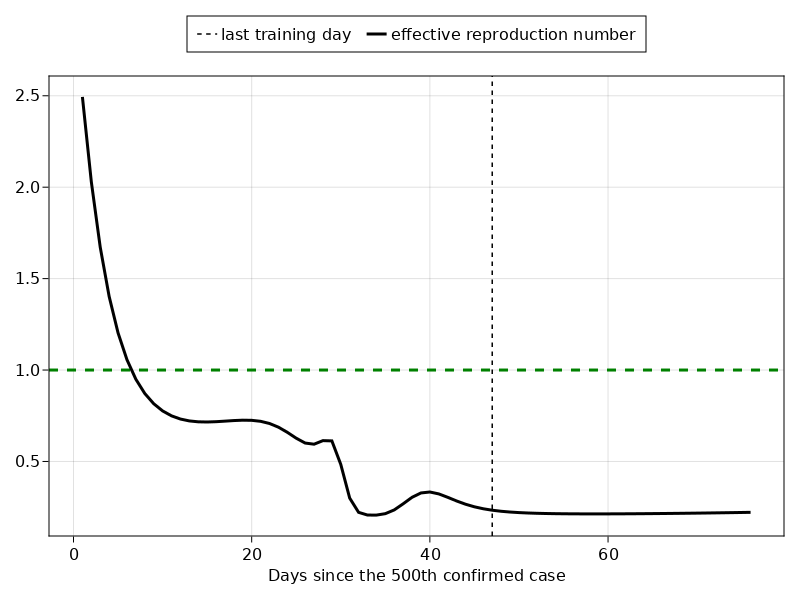
\includegraphics[width=\linewidth]{baseline/binhduong/20211216111951.baseline.binhduong.R_effective.png}
        \end{subfigure}
        \begin{subfigure}[b]{0.4\linewidth}
            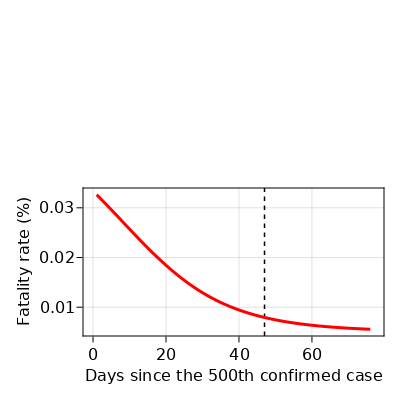
\includegraphics[width=\linewidth]{baseline/binhduong/20211216111951.baseline.binhduong.fatality_rate.png}
        \end{subfigure}
        \subcaption{Baseline model}
    \end{subfigure}

    \begin{subfigure}[b]{\linewidth}
        \centering
        \begin{subfigure}[b]{0.4\linewidth}
            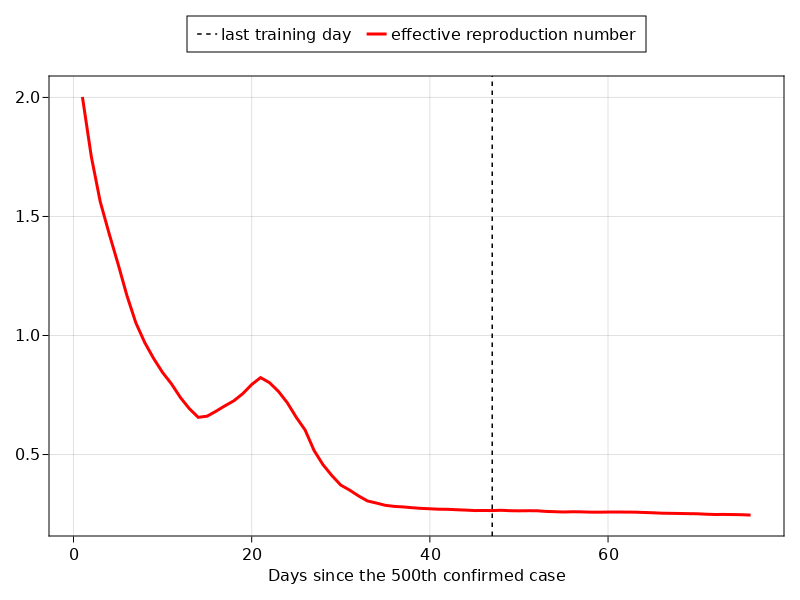
\includegraphics[width=\linewidth]{fb1/binhduong/20211216173307.fbmobility1.binhduong.R_effective.png}
        \end{subfigure}
        \begin{subfigure}[b]{0.4\linewidth}
            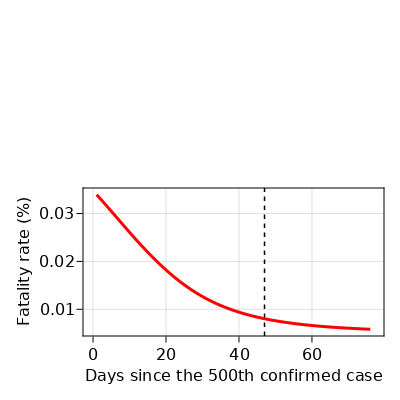
\includegraphics[width=\linewidth]{fb1/binhduong/20211216173307.fbmobility1.binhduong.fatality_rate.png}
        \end{subfigure}
        \subcaption{2nd. version}
    \end{subfigure}

    \begin{subfigure}[b]{\linewidth}
        \centering
        \begin{subfigure}[b]{0.4\linewidth}
            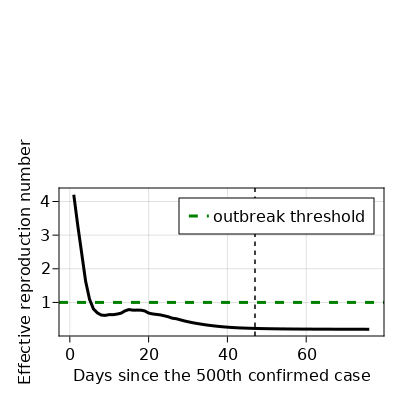
\includegraphics[width=\linewidth]{fb2/binhduong/20211216172741.fbmobility2.binhduong.R_effective.png}
        \end{subfigure}
        \begin{subfigure}[b]{0.4\linewidth}
            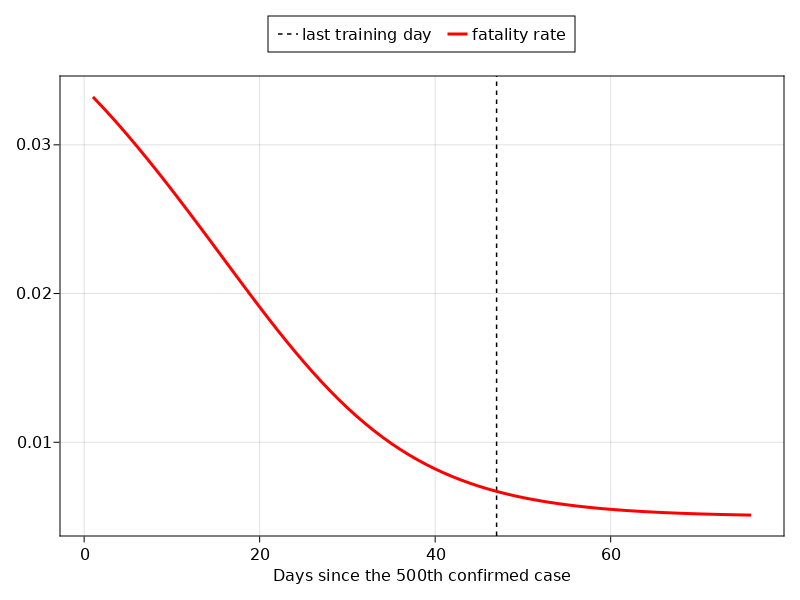
\includegraphics[width=\linewidth]{fb2/binhduong/20211216172741.fbmobility2.binhduong.fatality_rate.png}
        \end{subfigure}
        \subcaption{3rd. version}
    \end{subfigure}

    \caption{The effective reproduction number and the fatality rate for Binh Duong learned by different versions of the model}
    \label{fig:R0-and-fatality-binhduong}
\end{figure}

Looking at \autoref{fig:R0-and-fatality-dongnai}, it can be seen that all three versions predicted a similar trend for the fatality rate for Dong Nai.
In all versions, the fatality rate started at its maximum at the 0th time step and gradually decreased until the end of the simulation.
With the baseline model and the third version, the maximum fatality rate was predicted to be around $3$, while the second version predicted a higher fatality rate of $3.5$.
For the effective reproduction number, all three models also showed similar trends with slight differences in the first 20 time steps.
With the baseline model and the second version, the effective reproduction number started at its maximum value of $4.5$ and dropped drastically to below $1$ at around the 5th time step.
After that, the effective reproduction number increased for about 5 time steps to a value slightly above one before starting to decrease and stabilize.
With the third version, the effective reproduction number at time step 0 was the same as in the case with the other two versions, however, the value sharply dropped to below 1 at around the 10th time step and started to stabilize without experiencing an increase.

\begin{figure}[!htb]
    \centering

    \begin{subfigure}[b]{\linewidth}
        \centering
        \begin{subfigure}[b]{0.4\linewidth}
            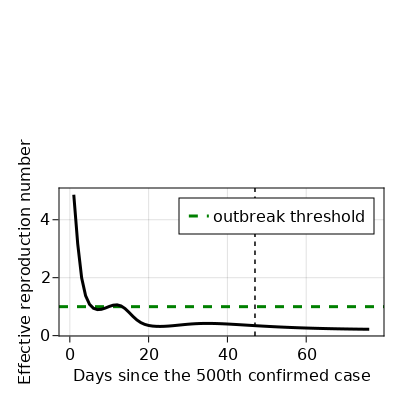
\includegraphics[width=\linewidth]{baseline/dongnai/20211216211601.baseline.dongnai.R_effective.png}
        \end{subfigure}
        \begin{subfigure}[b]{0.4\linewidth}
            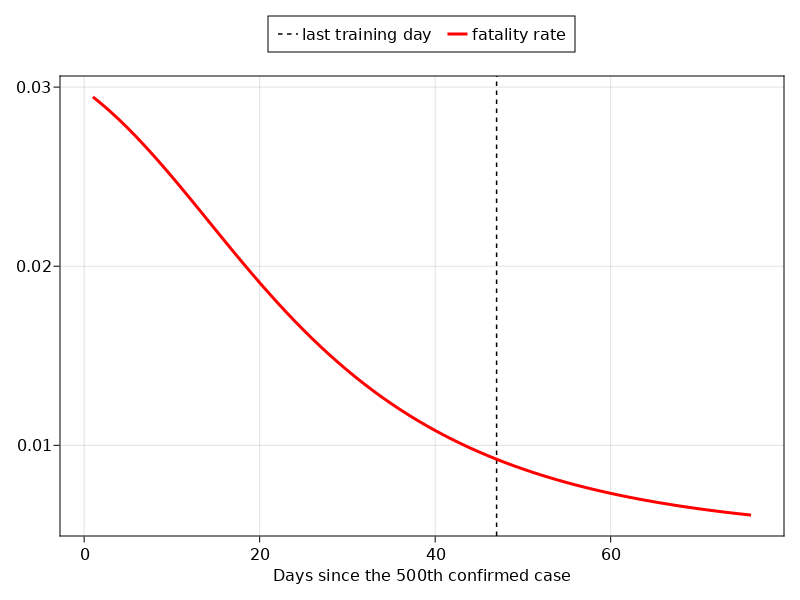
\includegraphics[width=\linewidth]{baseline/dongnai/20211216211601.baseline.dongnai.fatality_rate.png}
        \end{subfigure}
        \subcaption{Baseline model}
    \end{subfigure}

    \begin{subfigure}[b]{\linewidth}
        \centering
        \begin{subfigure}[b]{0.4\linewidth}
            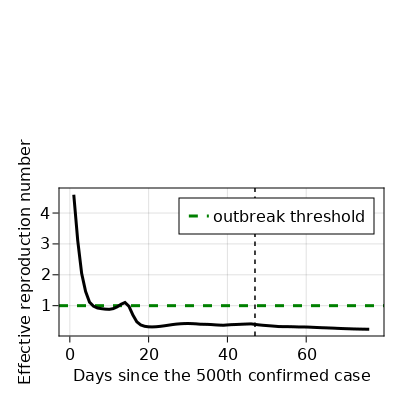
\includegraphics[width=\linewidth]{fb1/dongnai/20211216131821.fbmobility1.dongnai.R_effective.png}
        \end{subfigure}
        \begin{subfigure}[b]{0.4\linewidth}
            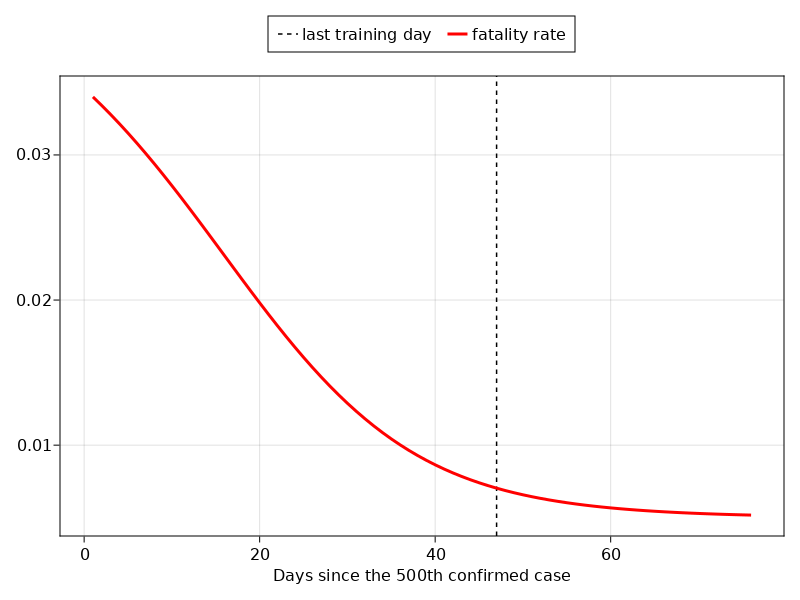
\includegraphics[width=\linewidth]{fb1/dongnai/20211216131821.fbmobility1.dongnai.fatality_rate.png}
        \end{subfigure}
        \subcaption{2nd. version}
    \end{subfigure}

    \begin{subfigure}[b]{\linewidth}
        \centering
        \begin{subfigure}[b]{0.4\linewidth}
            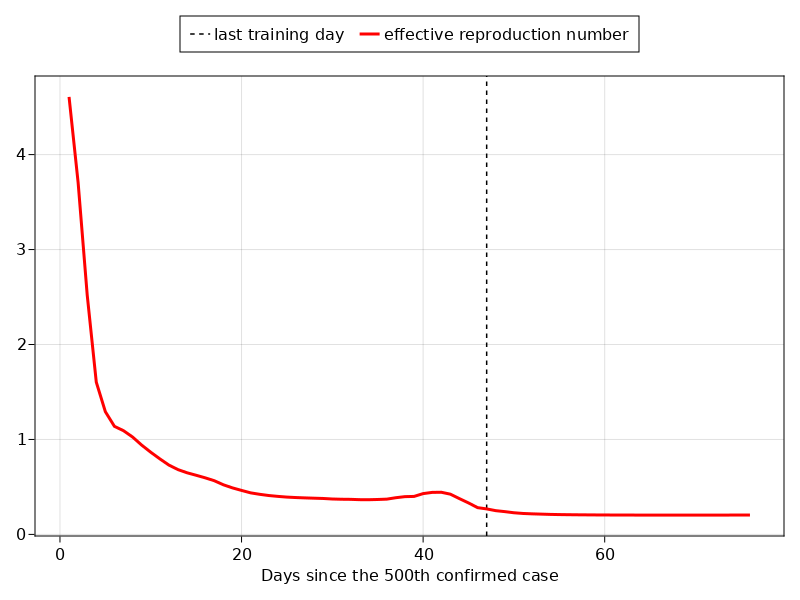
\includegraphics[width=\linewidth]{fb2/dongnai/20211217220549.fbmobility2.dongnai.R_effective.png}
        \end{subfigure}
        \begin{subfigure}[b]{0.4\linewidth}
            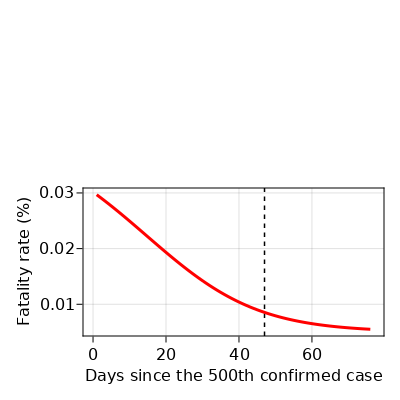
\includegraphics[width=\linewidth]{fb2/dongnai/20211217220549.fbmobility2.dongnai.fatality_rate.png}
        \end{subfigure}
        \subcaption{3rd. version}
    \end{subfigure}

    \caption{The effective reproduction number and the fatality rate for Dong Nai learned by different versions of the model}
    \label{fig:R0-and-fatality-dongnai}
\end{figure}

For Ho Chi Minh city, \autoref{fig:R0-and-fatality-hochiminh} showed that all versions predicted the same trend for both the fatality rate and the effective reproduction number.
The predicted effective reproduction number from all three versions fluctuated between $1.25$ and $1.5$ in the first 25 time steps before decreasing exponentially and stabilizing at around $0.25$ until the end of the simulation.
When predicting the fatality rate, all three versions showed an increasing trend that started from around $0.005$ at the 0th time step and increased to around $0.04$.
With the third version, the maximum predicted fatality rate was just below $0.04$ while the other two versions predicted a higher value of around $4.5$.

\begin{figure}[!htb]
    \centering

    \begin{subfigure}[b]{\linewidth}
        \centering
        \begin{subfigure}[b]{0.4\linewidth}
            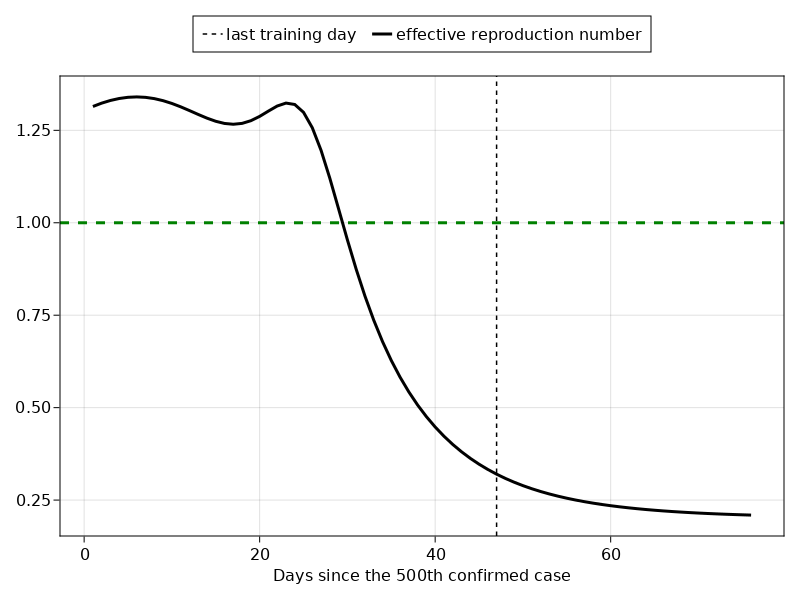
\includegraphics[width=\linewidth]{baseline/hcm/20211216154445.baseline.hcm.R_effective.png}
        \end{subfigure}
        \begin{subfigure}[b]{0.4\linewidth}
            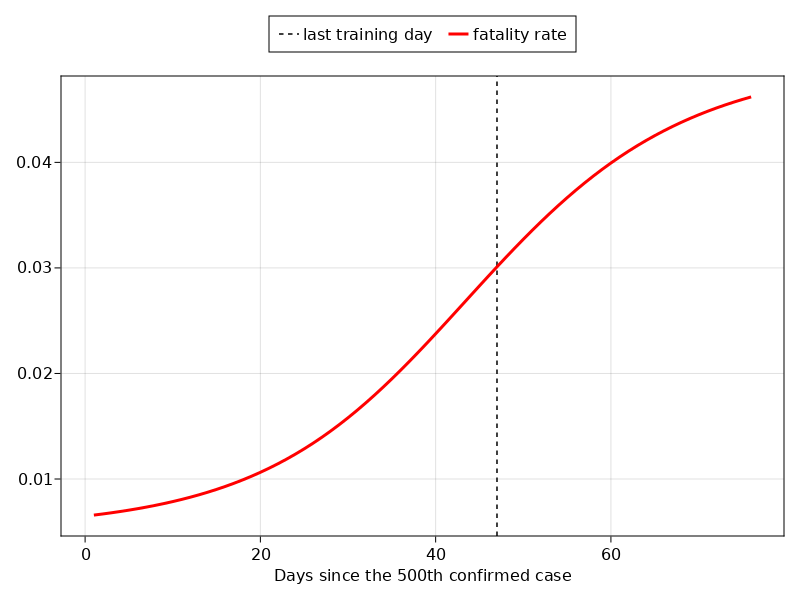
\includegraphics[width=\linewidth]{baseline/hcm/20211216154445.baseline.hcm.fatality_rate.png}
        \end{subfigure}
        \subcaption{Baseline model}
    \end{subfigure}

    \begin{subfigure}[b]{\linewidth}
        \centering
        \begin{subfigure}[b]{0.4\linewidth}
            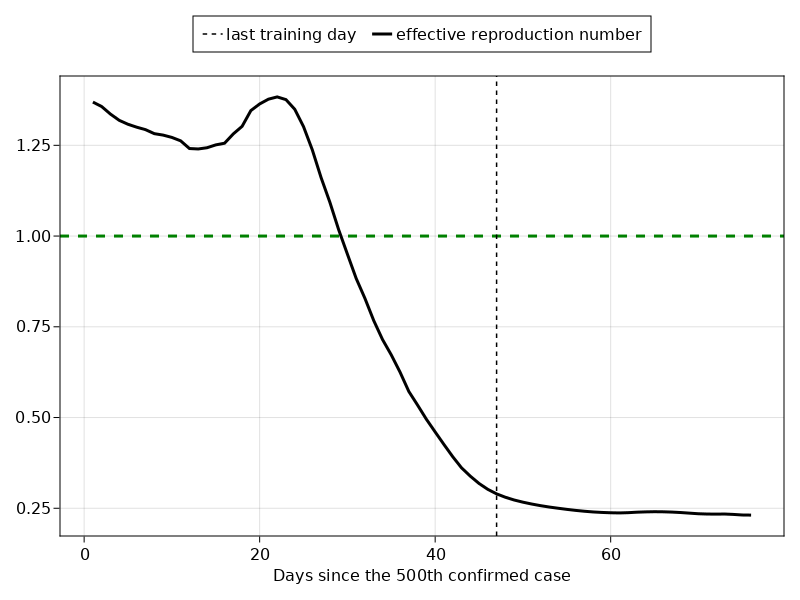
\includegraphics[width=\linewidth]{fb1/hcm/20211216231719.fbmobility1.hcm.R_effective.png}
        \end{subfigure}
        \begin{subfigure}[b]{0.4\linewidth}
            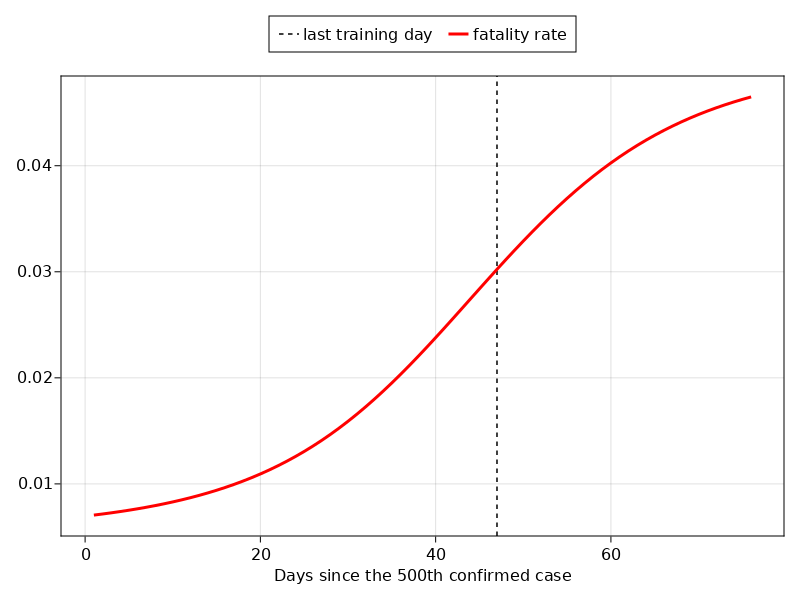
\includegraphics[width=\linewidth]{fb1/hcm/20211216231719.fbmobility1.hcm.fatality_rate.png}
        \end{subfigure}
        \subcaption{2nd. version}
    \end{subfigure}

    \begin{subfigure}[b]{\linewidth}
        \centering
        \begin{subfigure}[b]{0.4\linewidth}
            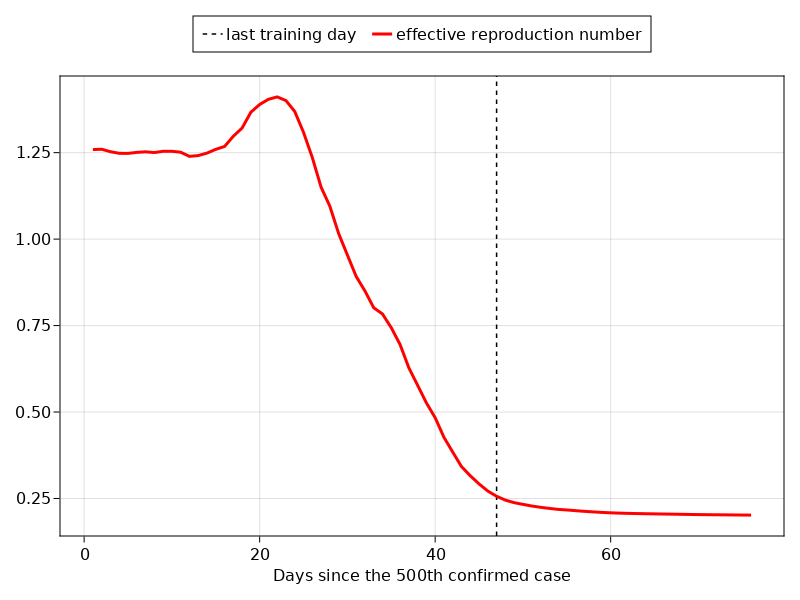
\includegraphics[width=\linewidth]{fb2/hcm/20211216183635.fbmobility2.hcm.R_effective.png}
        \end{subfigure}
        \begin{subfigure}[b]{0.4\linewidth}
            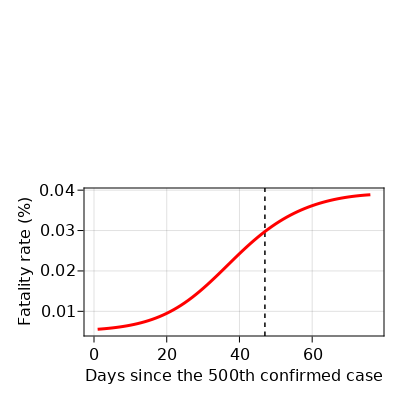
\includegraphics[width=\linewidth]{fb2/hcm/20211216183635.fbmobility2.hcm.fatality_rate.png}
        \end{subfigure}
        \subcaption{3rd. version}
    \end{subfigure}

    \caption{The effective reproduction number and the fatality rate for Ho Chi Minh city learned by different versions of the model}
    \label{fig:R0-and-fatality-hochiminh}
\end{figure}

Finally, for Long An, \autoref{fig:R0-and-fatality-longan} showed that the baseline model and the second version learned the same decreasing trend for the fatality rate while the third version learned an increasing trend.
The fatality rate predicted by the baseline model started at its highest of around $0.032$ at the 0th time step and gradually decreased to its minimum at around $0.026$.
With the second version, the fatality rate started at a higher maximum of $0.04$ at the 0th time step and gradually decreased to a lower minimum that was slightly above $0.01$
In contrast, the third version predicted a minimum fatality rate of around $0.01$ at the 0th time step that gradually increased to a maximum of $0.04$.
Because of these differences, the resulting dynamics for the deaths compartment from these versions were also highly different from each other.
Looking at \autoref{fig:fit-vn-provinces} and \autoref{fig:pred-vn-provinces}, we can see that the second version had a much better fit to the training data and can extrapolate with high accuracy, while both the baseline model and the third version fitted poorly to training data and overestimated the number of deaths when extrapolated into the future.
For the effective reproduction number, all versions predicted a low initial value that surged to a maximum after 5 time steps.
With the baseline model, a maximum effective reproduction number of around $2.5$ was predicted, and once the max value was reached, the effective reproduction decreased exponentially and crossed the $1$ threshold at around the 20th time steps.
On the other hand, both the second version and the third version predicted a maximum effective reproduction number of around $4$ where the value predicted by the second version was slightly lower than $4$ and the value predicted by the third version was slightly higher than $4$.
Once the maximum was reached, the predicted effective reproduction number in both versions dropped significantly and crossed the $1$ threshold at around the 15th time step.
Finally, the predicted effective reproduction number raised slightly and reached the $1$ threshold at around the 20th time step before finally decreasing for the rest of the simulated period.

\begin{figure}[!htb]
    \centering

    \begin{subfigure}[b]{\linewidth}
        \centering
        \begin{subfigure}[b]{0.4\linewidth}
            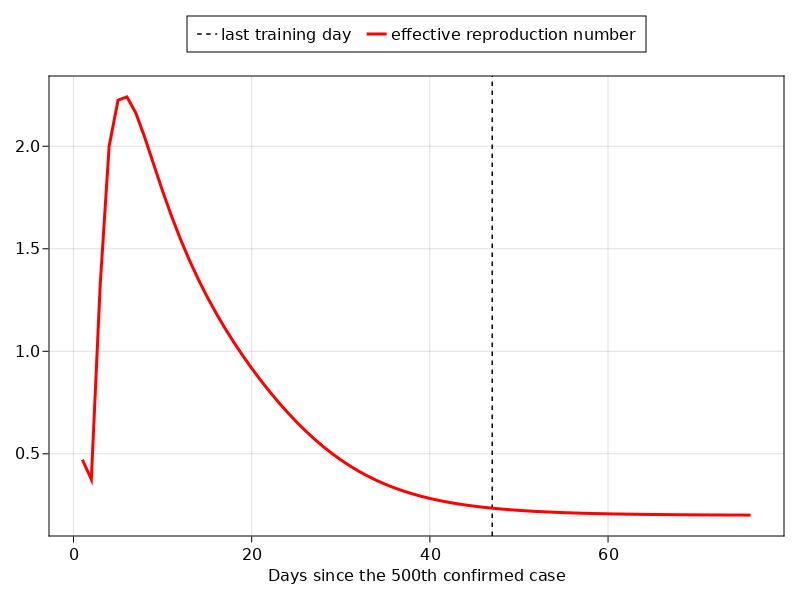
\includegraphics[width=\linewidth]{baseline/longan/20211216111951.baseline.longan.R_effective.png}
        \end{subfigure}
        \begin{subfigure}[b]{0.4\linewidth}
            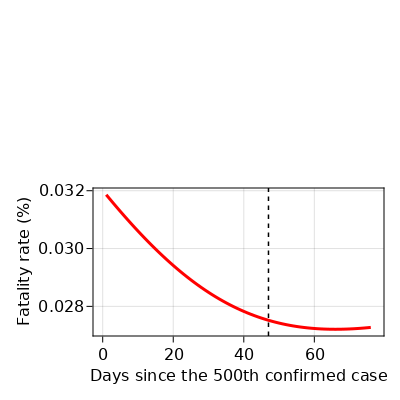
\includegraphics[width=\linewidth]{baseline/longan/20211216111951.baseline.longan.fatality_rate.png}
        \end{subfigure}
        \subcaption{Baseline model}
    \end{subfigure}

    \begin{subfigure}[b]{\linewidth}
        \centering
        \begin{subfigure}[b]{0.4\linewidth}
            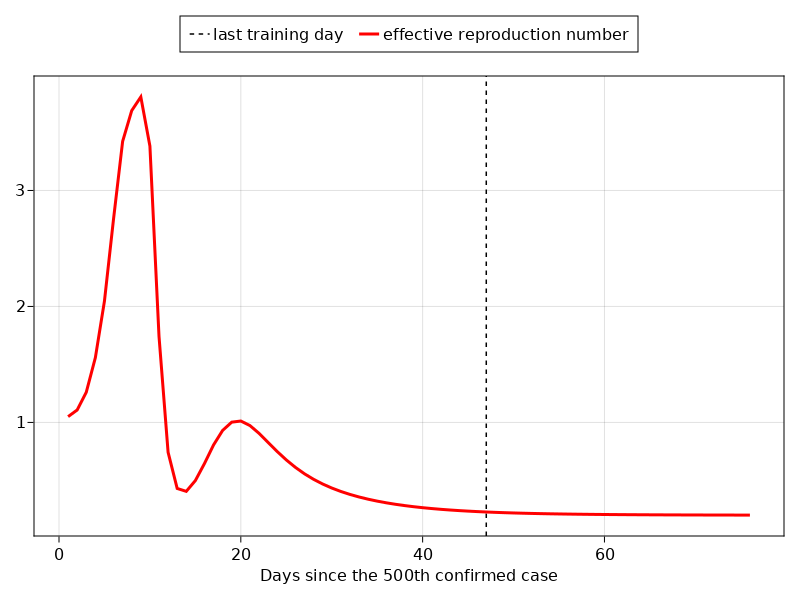
\includegraphics[width=\linewidth]{fb1/longan/20211216131821.fbmobility1.longan.R_effective.png}
        \end{subfigure}
        \begin{subfigure}[b]{0.4\linewidth}
            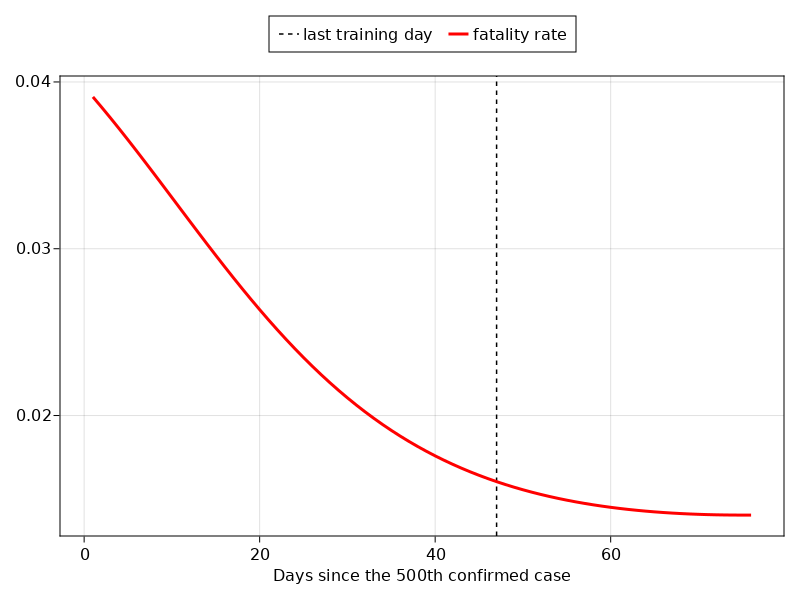
\includegraphics[width=\linewidth]{fb1/longan/20211216131821.fbmobility1.longan.fatality_rate.png}
        \end{subfigure}
        \subcaption{2nd. version}
    \end{subfigure}

    \begin{subfigure}[b]{\linewidth}
        \centering
        \begin{subfigure}[b]{0.4\linewidth}
            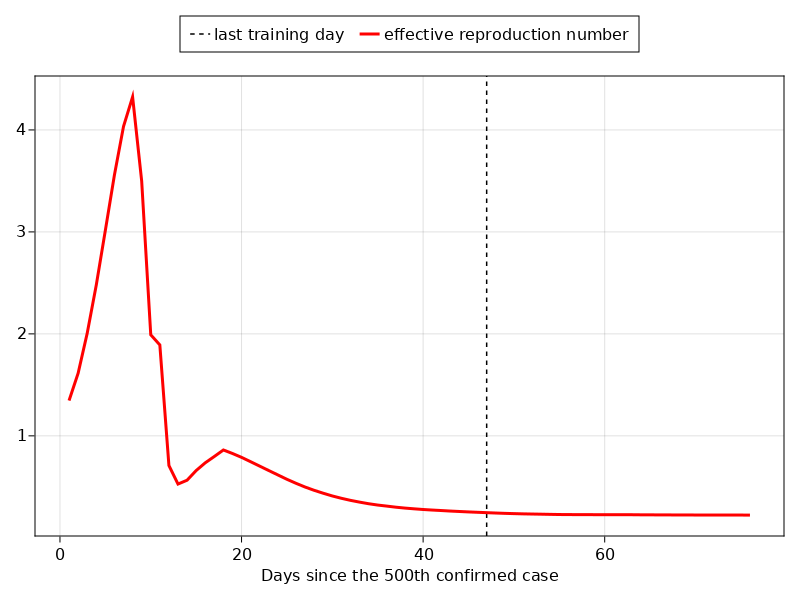
\includegraphics[width=\linewidth]{fb2/longan/20211216193717.fbmobility2.longan.R_effective.png}
        \end{subfigure}
        \begin{subfigure}[b]{0.4\linewidth}
            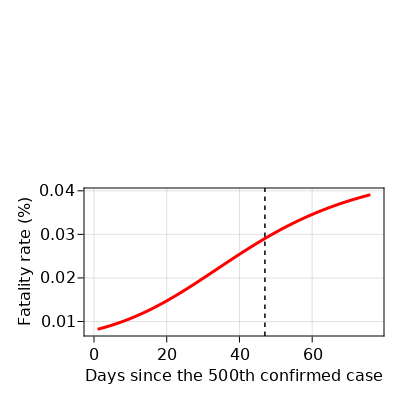
\includegraphics[width=\linewidth]{fb2/longan/20211216193717.fbmobility2.longan.fatality_rate.png}
        \end{subfigure}
        \subcaption{3rd. version}
    \end{subfigure}

    \caption{The effective reproduction number and the fatality rate for Long An learned by different versions of the model}
    \label{fig:R0-and-fatality-longan}
\end{figure}
